\subsection{Les téléphones}
Cette partie permet de voir la liste des téléphones, éditer leurs configurations et les acheter.

\subsubsection{Consulter la liste des téléphones}
Cette action est disponible pour tous les types d'utilisateurs. Pour cela, il suffit de cliquer sur la lignes \og Les téléphones\fg{} de la barre de menu. On aboutit alors à l'interface de la Figure~\ref{fig:phones-list}.

\begin{figure}[ht]
  \centering
  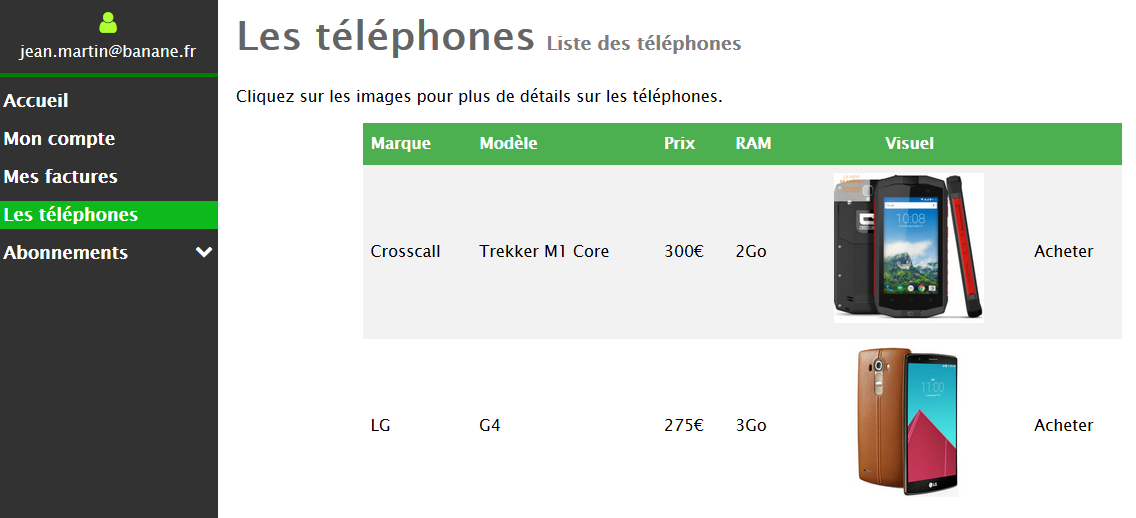
\includegraphics[width=.7\textwidth]{images/Plateforme/phone-list}
  \caption{Consulter la liste des téléphones}
  \label{fig:phones-list}
\end{figure}

On remarquera que cette liste ne propose pas initialement toutes les caractéristiques des téléphones. Afin d'accéder à ces dernières, l'utilisateur doit cliquer sur l'image du téléphone. Une modale avec tous les détails apparaît alors, comme proposée à la Figure~\ref{fig:phone-details}.

\begin{figure}[ht]
  \centering
  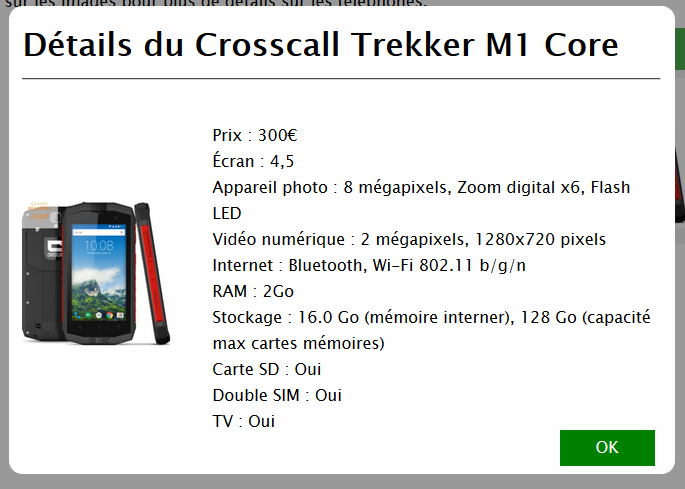
\includegraphics[width=.7\textwidth]{images/Plateforme/phone-details}
  \caption{Affichage des détails d'un téléphone}
  \label{fig:phones-details}
\end{figure}

\subsubsection{Créer et modifier un téléphone}
Ces actions ne peuvent être réalisées que par un administrateur.
\subParagraphe{Créer un nouveau téléphone}Pour cela, un administrateur doit simplement cliquer sur le bouton \og Nouvel appareil\fg. Une modale s'ouvre alors, lui proposant de remplir tous les champs permettant de caractériser le téléphone. Cette modale vous est proposée à la Figure~\ref{fig:new-phone}.

\begin{figure}[ht]
  \centering
  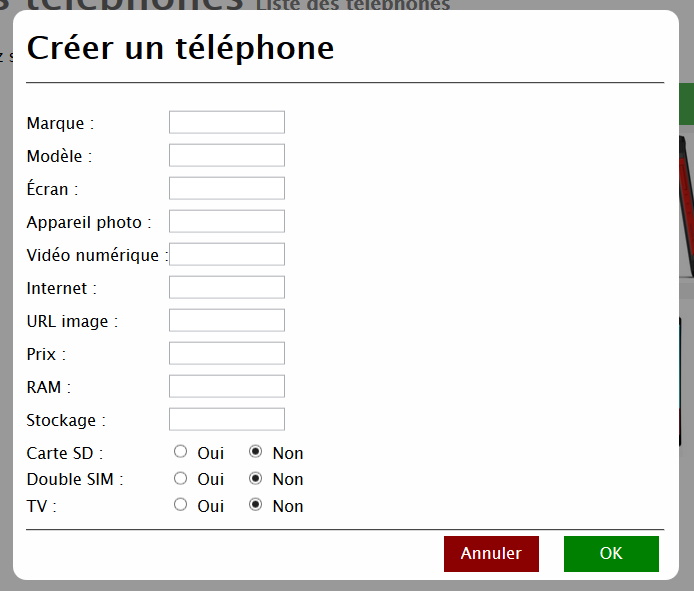
\includegraphics[width=.5\textwidth]{images/Plateforme/new_phone}
  \caption{Création d'un téléphone}
  \label{fig:new-phone}
\end{figure}

Si en cliquant sur \og OK\fg, la table n'est pas mis à jour, c'est que certains champs obligatoires n'ont pas été remplis. Sinon, tous les champs remplis sont corrects.

\subParagraphe{\'Edition d'un téléphone}De manière transparente, l'administrateur peut cliquer sur l'icône \vColor{\faEdit} d'un téléphone. Une modale de même aspect que celle de la Figure~\ref{fig:new-phone} apparaît alors avec les valeurs pré-remplies du téléphone. L'administrateur peut alors éditer ces valeurs à loisir.

\subParagraphe{Suppresion d'un téléphone}Cette dernière se fait en cliquant sur l'icône \thColor{\faRemove} du téléphone. Ce dernier n'est alors pas supprimé entièrement de la base de données. Il est supprimé des formules qui le proposait auparavant, et son champ \texttt{is\_deleted} qui représente sa mise sur le marché est mis à \texttt{TRUE}, pour que ce dernier n'apparaisse plus dans les listes de téléphones. Il n'est cependant pas totalement supprimé de la base de données, pour que les utilisateurs l'ayant acheté le voit toujours apparaître dans leur liste d'achat.

\subsubsection{Achter un téléphone}
Cette action ne peut être réalisée que par un client. Pour cela, ce dernier dispose de la possibilité de cliquer sur la case \og Acheter\fg{} à la fin de chaque ligne de la table présentant les téléphones. En faisant ainsi, une modale s'ouvre pour valider la commande, comme présentée à la Figure~\ref{fig:achat-phone}.

\begin{figure}[ht]
  \centering
  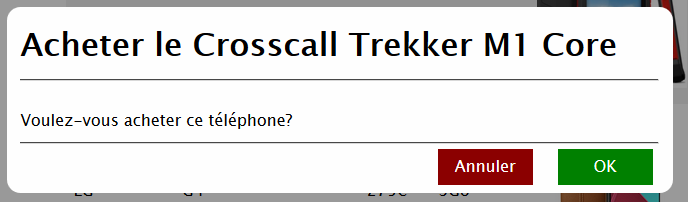
\includegraphics[width=.6\textwidth]{images/Plateforme/buy_phone}
  \caption{Confirmation de l'achat d'un téléphone}
  \label{fig:achat-phone}
\end{figure}

En cliquant sur \og OK\fg, le client valide alors la commande, il peut annuler l'action en cliquant sur \og Annuler\fg. La consultation de la liste des téléphones achetés sera détaillée plus loin dans la partie consacrée aux abonnements.



%%% Local Variables:
%%% mode: latex
%%% TeX-master: "../../Rapport_BDD"
%%% End:
